\documentclass[utf8]{FrontiersinHarvard}

% -------------------------------------------------------
% PACKAGES
% -------------------------------------------------------
\usepackage{url}
\usepackage{hyperref}
\usepackage{lineno}
\usepackage{microtype}
\usepackage{subcaption}
\usepackage[onehalfspacing]{setspace}
\usepackage{booktabs}
\usepackage{siunitx}
\sisetup{detect-all}
\usepackage{tabularx}
\usepackage{float}
\usepackage[dvipsnames]{xcolor}
\usepackage{pgfplots}
\pgfplotsset{compat=1.18}
\usepackage{tikz}
\usetikzlibrary{arrows.meta, positioning, shapes.geometric, fit, backgrounds}
\usepackage{amsmath}
\usepackage{amssymb}
\usepackage{enumitem}
\usepackage{multirow}

\newcolumntype{Y}{>{\centering\arraybackslash}X}

\hypersetup{
	colorlinks=true,
	linkcolor=MidnightBlue,
	urlcolor=MidnightBlue,
	citecolor=MidnightBlue
}

\linenumbers

% -------------------------------------------------------
% FRONTIERS METADATA
% -------------------------------------------------------
\def\firstAuthorLast{Syed et~al.}

\def\Authors{
	Toqeer Ali Syed$^{1}$,
	Hatem M.\ El-Boghdadi$^{1}$,
	Muhammad Tayyab Naqash$^{2,*}$,
	Turki Alghamdi$^{1}$,
	Abdulaziz Alshahrani$^{1}$,
	It Ee Lee$^{3}$,
	Ali Akarma$^{1}$
}

\def\Address{
	$^{1}$Faculty of Computer and Information Systems, Islamic University of Madinah,
	Madinah 42351, Saudi Arabia\\
	$^{2}$Civil Engineering Department, Islamic University of Madinah,
	Madinah 42351, Saudi Arabia\\
	$^{3}$Faculty of Artificial Intelligence, Multimedia University,
	Selangor 63100, Malaysia
}

\def\corrAuthor{Muhammad Tayyab Naqash}
\def\corrEmail{mnaqash@iu.edu.sa}

% -------------------------------------------------------
\begin{document}
	\onecolumn
	\firstpage{1}

	\title[Agentic Commerce]{Agentic Commerce: Economic Implications of
		AI-Driven Forecasting, Inventory Management, and Product
		Personalization in Retail}

	\author[\firstAuthorLast]{\Authors}
	\address{}
	\correspondance{}
	\extraAuth{}

	\maketitle

	% -------------------------------------------------------
	\begin{abstract}

	Retail marts with broad product assortments face persistent challenges in
	maintaining optimal stock levels, responding to volatile demand, and
	identifying high-potential new products across heterogeneous categories.
	Traditional inventory control methods---such as static Economic Order
	Quantity (EOQ) and Reorder Point (ROP) policies---rely on fixed thresholds
	and manual oversight, rendering them inadequate at the scale and velocity
	required by modern multi-category retail operations.  This paper proposes
	the \emph{Agentic AI Inventory Replenishment and Management} (AAIRM)
	framework: a multi-agent, LangChain-orchestrated system that implements
	autonomous inventory replenishment and product discovery through a structured
	Perception--Conceptualization--Action (PCA) workflow.  Perception agents
	continuously ingest sales, inventory, supplier, and external trend data.
	Conceptualization agents perform demand forecasting, reorder optimisation,
	supplier ranking, and governance enforcement.  Action agents execute
	purchase orders, interface with logistics systems, and sustain a
	continuous learning loop via reinforcement-learning policy updates.  The
	framework is evaluated against a structurally realistic synthetic simulation
	comprising 1\,200 SKUs across five product categories.  AAIRM achieves
	a stockout rate of 3.9\%, compared with 8.7\% for the classical ROP--EOQ
	baseline---a relative reduction of 55.2\%---while simultaneously reducing
	total operational cost by 16\% and raising the fill rate to 97.8\%.
	Supplier diversification improves markedly, with the diversification index
	rising from 0.42 to 0.61, indicating substantially lower single-source
	procurement risk.  These results demonstrate the economic viability and
	operational superiority of agentic AI as a foundation for self-governing,
	adaptive retail operations.

	\tiny
	\keyFont{\section{Keywords:}
		Agentic AI, inventory management, multi-agent systems, demand
		forecasting, supply chain optimisation, retail automation,
		reinforcement learning, LangChain}
	\end{abstract}

	% -------------------------------------------------------
	\section{Introduction}
	\label{sec:intro}

	Retail marts that carry diverse merchandise---spanning groceries, apparel,
	cosmetics, frozen foods, dry fruits, and children's clothing---operate in
	intensely competitive and demand-volatile markets.  Irregular consumption
	patterns, short product life cycles, supplier unreliability, and the
	perishable nature of many goods make it exceptionally difficult to maintain
	optimal inventory levels across thousands of stock-keeping units (SKUs)
	simultaneously.  The economic consequences are substantial: McKinsey
	estimates that global retailers lose over \$1.8 trillion annually due to
	stockouts, overstocking, and associated inefficiencies in forecasting and
	replenishment \cite{mckinsey2024retailai}.  Despite this, approximately
	62\% of retailers continue to rely on manual or spreadsheet-based
	replenishment practices rather than data-driven systems
	\cite{capgemini2023autonomous}.

	Conventional inventory control methods---including the Economic Order
	Quantity (EOQ) and Reorder Point (ROP) models---apply fixed thresholds
	and demand-averaged parameters that are calibrated offline and updated
	infrequently.  These approaches break down in large-scale retail
	environments characterised by thousands of SKUs with heterogeneous lead
	times, irregular shelf lives, and non-stationary demand.  In fragmented,
	fast-moving supply networks, fixed-threshold policies cannot deliver the
	responsiveness and cost-effectiveness demanded by modern retail supply
	chains \cite{bullwhip2007effect}.

	Recent advances in artificial intelligence (AI) and autonomous digital
	agents offer a fundamentally different paradigm.  \emph{Agentic AI
	systems}---software agents capable of perception, reasoning,
	decision-making, and autonomous negotiation---enable intelligent
	replenishment that adapts in real time.  Large language models (LLMs),
	predictive analytics, and reinforcement learning can be combined to
	automate ordering decisions, optimise procurement, and engage dynamically
	with supplier systems.  Jannelli et al.\ \cite{jannelli2024agentic}
	demonstrated that multi-agent LLM-based coordination can produce material
	improvements in procurement-cycle efficiency.  Culot et al.\
	\cite{culot2024ai} further showed that AI-enhanced supply chains improve
	transparency, demand accuracy, and operational agility.  Nevertheless,
	existing approaches tend to address isolated sub-problems---forecasting,
	ordering, or supplier selection---rather than providing an integrated,
	end-to-end autonomous replenishment pipeline.

	This gap is especially acute in multi-category retail settings, where a
	cohesive system must simultaneously discover emergent product trends,
	monitor on-hand inventory, forecast cross-category demand, initiate
	supplier negotiations, and execute procurement---all within a coordinated
	decision architecture.  To address this challenge, this paper proposes
	the \emph{AAIRM framework}: an agentic AI platform for autonomous inventory
	replenishment and product discovery in multi-category retail marts.  The
	framework coordinates specialised agents across three functional layers:
	Perception, Conceptualization, and Action.  The principal contributions
	are as follows:

	\begin{itemize}[leftmargin=*]
		\item A unified agentic architecture that integrates trend discovery,
		inventory monitoring, demand forecasting, supplier selection,
		autonomous negotiation, and replenishment execution within a single
		Perception--Conceptualization--Action workflow.

		\item A multi-objective optimisation formulation that simultaneously
		balances procurement cost, supplier diversification, perishability
		constraints, and target service levels.

		\item Empirical evaluation on a structurally realistic synthetic
		simulation demonstrating significant improvements in stockout rate,
		total cost, fill rate, and cross-category inventory stability
		relative to classical and machine-learning baselines.

		\item A discussion of deployment considerations---including LLM
		inference latency, supplier API interoperability, human-AI
		governance, and the economic implications of agentic procurement
		automation---that contextualises the framework for real-world
		adoption.
	\end{itemize}

	The remainder of the paper is structured as follows.
	Section~\ref{sec:background} provides theoretical and technological
	background.  Section~\ref{sec:related} reviews related work.
	Section~\ref{sec:framework} presents the proposed architecture.
	Section~\ref{sec:impl} describes the experimental setup and results.
	Section~\ref{sec:discussion} discusses implications and limitations.
	Section~\ref{sec:conclusion} concludes with directions for future
	research.

	% -------------------------------------------------------
	\section{Background}
	\label{sec:background}

	This section establishes the theoretical and technological foundations
	of the proposed framework, covering classical inventory theory,
	AI-driven supply chain management, and the emerging paradigm of
	agentic AI systems.

	\subsection{Inventory Models and Reorder Policies}

	Classical inventory theory governs stocking and replenishment decisions
	through well-established constructs: the Economic Order Quantity (EOQ),
	safety stock sizing, lead-time buffering, and the Reorder Point (ROP)
	\cite{nahmias2019production}.  The canonical ROP formulation is
	\begin{equation}
		\label{eq:rop}
		\text{ROP} = \mu_D \cdot L + z \cdot \sigma_D \sqrt{L},
	\end{equation}
	where $L$ is the replenishment lead time (in periods), $z$ is the
	safety factor corresponding to the target service level, and $\mu_D$
	and $\sigma_D$ are the mean and standard deviation of demand per unit
	time, respectively.  Equation~(\ref{eq:rop}) ensures sufficient stock
	to absorb both predictable and stochastic demand during the
	replenishment cycle, but it requires accurate and stationary estimates
	of $\mu_D$ and $\sigma_D$---an assumption that rarely holds in
	multi-category retail.

	Modern supply chains extend beyond single-echelon systems to networked
	structures involving multiple warehouses, suppliers, and retail outlets.
	Multi-echelon and joint-replenishment frameworks account for
	upstream-downstream information flows and coordination mechanisms
	\cite{axsater2015inventory}.  A well-known pathology of such networks
	is the \emph{bullwhip effect}: small fluctuations in customer demand
	amplify progressively upstream, producing costly production and inventory
	oscillations \cite{bullwhip2007effect}.  Mitigation strategies include
	information-sharing contracts and Collaborative Planning, Forecasting and
	Replenishment (CPFR), which align decision-making across supply-chain
	partners \cite{sari2008collaborative}.  Perishable product categories
	add a further dimension of complexity, as expiration dates impose hard
	capacity constraints on safety-stock policies \cite{nahmias1982perishable,
	karaesmen2011perishable}.

	\subsection{AI in Supply Chain and Inventory Management}

	Artificial intelligence has reshaped demand forecasting, procurement,
	and replenishment in supply chain research.  Time-series models,
	regression techniques, and deep learning architectures are effective at
	capturing non-stationary demand and informing timely procurement decisions
	\cite{culot2024ai}.  Machine learning coupled with optimisation has been
	shown to reduce stockouts and holding costs by continuously updating reorder
	criteria from real-time data streams \cite{yilmaz2024aiinventory}.  In
	particular, Long Short-Term Memory (LSTM) and Transformer architectures
	have emerged as primary drivers of next-generation demand planning
	\cite{shukla2023review}.

	The deployment of IoT sensors and edge analytics has further enabled
	autonomous, event-driven replenishment systems \cite{duan2022iot}.
	Reinforcement learning (RL) has attracted particular interest as a
	mechanism for experience-driven policy adaptation, replacing fixed
	heuristics with learned ordering strategies.  Chen and Zhang
	\cite{chen2020multiproduct} demonstrated multi-agent RL for coordinating
	replenishment across multiple nodes and SKUs; Siems and Peters
	\cite{siems2023interpretable} proposed interpretable RL policies for
	dynamic ordering under non-stationary demand.  Both approaches outperform
	classical methods when demand patterns and lead times are uncertain.

	\subsection{Emerging Agentic AI in Supply Chains}

	The most recent research frontier is \emph{agentic AI}: autonomous,
	reasoning-capable software agents that perceive complex environments,
	form plans, and act across distributed supply-chain systems.  Unlike
	classical AI modules that operate as isolated components, agentic systems
	communicate, delegate tasks, and pursue composite goals through structured
	inter-agent coordination.

	Jannelli et al.\ \cite{jannelli2024agentic} introduced an LLM-based
	agentic framework in which supply-chain participants negotiate and
	coordinate procurement decisions through natural-language reasoning---a
	significant step toward self-managing supply chains that merge strategic
	planning with predictive intelligence.  This line of research directly
	motivates the multi-agent design proposed here, which extends autonomous
	monitoring and ordering into a coordinated ecosystem spanning forecasting,
	supplier identification, negotiation, and execution.

	% -------------------------------------------------------
	\section{Literature Review}
	\label{sec:related}

	Existing literature relevant to this work falls into three streams:
	(i)~multi-category and perishable inventory management, (ii)~agentic and
	autonomous supply-chain frameworks, and (iii)~AI and machine learning for
	inventory optimisation and procurement.  Table~\ref{tab:litreview}
	summarises the positioning of this work relative to key prior contributions.

	\begin{table}[htbp]
		\centering
		\caption{Positioning of the proposed AAIRM framework relative to
			representative prior work across the three literature streams.
			\checkmark~indicates full support; $\circ$~indicates partial
			support; \textemdash~indicates the property is absent.}
		\label{tab:litreview}
		\begin{tabularx}{\linewidth}{Xcccc}
			\toprule
			\textbf{Work} &
			\textbf{Multi-category} &
			\textbf{Agentic coord.} &
			\textbf{RL policy} &
			\textbf{Supplier negot.} \\
			\midrule
			Nahmias \cite{nahmias1982perishable}           & $\circ$ & \textemdash & \textemdash & \textemdash \\
			Shen \& Norrie \cite{shen1999multiagent}       & $\circ$ & \checkmark  & \textemdash & \textemdash \\
			Chen \& Zhang \cite{chen2020multiproduct}      & \checkmark & $\circ$  & \checkmark  & \textemdash \\
			Siems \& Peters \cite{siems2023interpretable}  & $\circ$ & \textemdash & \checkmark  & \textemdash \\
			Jannelli et al.\ \cite{jannelli2024agentic}    & \textemdash & \checkmark & \textemdash & \checkmark \\
			Yılmaz et al.\ \cite{yilmaz2024aiinventory}   & $\circ$ & \textemdash & \textemdash & \textemdash \\
			\textbf{AAIRM (this work)}                      & \checkmark & \checkmark & \checkmark  & \checkmark \\
			\bottomrule
		\end{tabularx}
	\end{table}

	\subsection{AI and Machine Learning for Inventory and Procurement}

	Artificial intelligence has become a central element of contemporary supply
	chain research.  Bhavikatta and Reddy \cite{bhavikatta2024survey} provide
	a comprehensive survey of AI-driven inventory optimisation, reporting that
	ML-based forecasting and optimisation consistently outperform rule-based
	baselines on responsiveness, accuracy, and scalability.  Culot et al.\
	\cite{culot2024ai} reviewed AI applications across supply-chain stages and
	found that data integration, interoperability, and model interpretability
	remain open challenges for industrial adoption.

	Yılmaz et al.\ \cite{yilmaz2024aiinventory} proposed a dynamic
	procurement model trained on historical sales and supplier reliability
	metrics, demonstrating measurable reductions in unsold inventory and
	stockout events.  Shukla and Bose \cite{shukla2023review} identified
	LSTM and Transformer architectures as the primary drivers of next-generation
	demand planning, deepening the role of deep learning in supply-chain
	predictive analytics.  Reinforcement learning has emerged as an effective
	decision-support paradigm for dynamic ordering: Siems and Peters
	\cite{siems2023interpretable} demonstrated interpretable RL policies for
	non-stationary demand environments, while Chen and Zhang
	\cite{chen2020multiproduct} showed that decentralised multi-agent RL
	outperforms fixed heuristic ordering rules in multi-node networks under
	uncertainty.  Collectively, these results establish the predictive and
	procurement merits of AI and ML; however, the approaches remain largely
	centralised, lacking the inter-agent reasoning and end-to-end autonomy
	that characterise the present work.

	\subsection{Agentic and Autonomous Frameworks in Supply Chains}

	Classical automation responds reactively to predefined triggers, whereas
	agentic AI introduces active, reasoning-based coordination among distributed
	supply-chain units.  Jannelli et al.\ \cite{jannelli2024agentic} were
	among the first to propose LLM-based agentic coordination in which
	supply-chain agents reason about procurement choices in natural language,
	replacing dynamic optimisation with autonomous negotiation and adaptive
	cooperation.

	Earlier multi-agent system (MAS) research established decentralised methods
	for logistics and order management.  Shen and Norrie
	\cite{shen1999multiagent} applied intelligent agents to scheduling and
	resource allocation in manufacturing supply chains, demonstrating that
	local decision autonomy can reduce global coordination costs.  Davidrajuh
	and Lin \cite{davidrajuh2018multiagent} proposed a multi-agent simulation
	for dynamic inventory balancing in stochastic environments.  These models
	reduced information asymmetry and maximised local decision autonomy;
	however, they predate modern LLM-driven decision tools that enable semantic
	negotiation, self-optimising procurement strategies, and trust evaluation.
	The present work builds directly on this MAS foundation while incorporating
	contemporary LLM and RL capabilities.

	\subsection{Multi-Category and Perishable Inventory Models}

	Much of the AI-driven inventory literature focuses on homogeneous or
	single-category product lines.  Perishable and category-diverse assortments
	introduce additional complexity through expiration modelling, cross-category
	priority structures, and heterogeneous margin structures.  Nahmias
	\cite{nahmias1982perishable} established foundational analytical models for
	perishable inventory control; Karaesmen et al.\ \cite{karaesmen2011perishable}
	extended these to stochastic multi-period settings with dynamic pricing and
	finite shelf lives.  More recently, IoT-enabled freshness tracking and
	predictive aging have improved perishable management at the individual item
	level \cite{duan2022iot}.  Vendor-managed inventory (VMI) systems address
	some cross-category coordination but rely heavily on supplier control and
	manual parameter adjustment \cite{sari2008collaborative}.

	The present work distinguishes itself from all prior contributions by
	providing a single multi-category framework in which autonomous agents
	forecast demand, negotiate contracts, and execute orders across both durable
	and perishable goods.  Crucially, AAIRM integrates autonomous
	decision-making, cross-category optimisation, and AI-based supplier
	reasoning---three dimensions largely absent from the existing literature
	in combination.

	% -------------------------------------------------------
	\section{Proposed Framework}
	\label{sec:framework}

	The AAIRM framework implements inventory replenishment, procurement, and
	product discovery through a structured Perception--Conceptualization--Action
	(PCA) workflow.  Figure~\ref{fig:pca-arch} illustrates the complete
	architecture, comprising four functional zones: the Perception and
	Intelligence Layer, the Cognitive Multi-Agent Planning Layer, the Execution
	and Operational Agents cluster, and the Trusted Agent Infrastructure.  A
	central \emph{Meta-Orchestrator} (implemented via LangGraph and LangChain)
	coordinates task decomposition, agent memory, and tool routing across all
	zones.  An External Commerce Ecosystem---spanning ERP and inventory
	databases, warehouse management systems (WMS), supplier and logistics APIs,
	marketplace platforms, and the e-commerce frontend---provides the operational
	interfaces through which agents perceive and act upon the physical retail
	environment.

	\begin{figure*}[htbp]
		\centering
		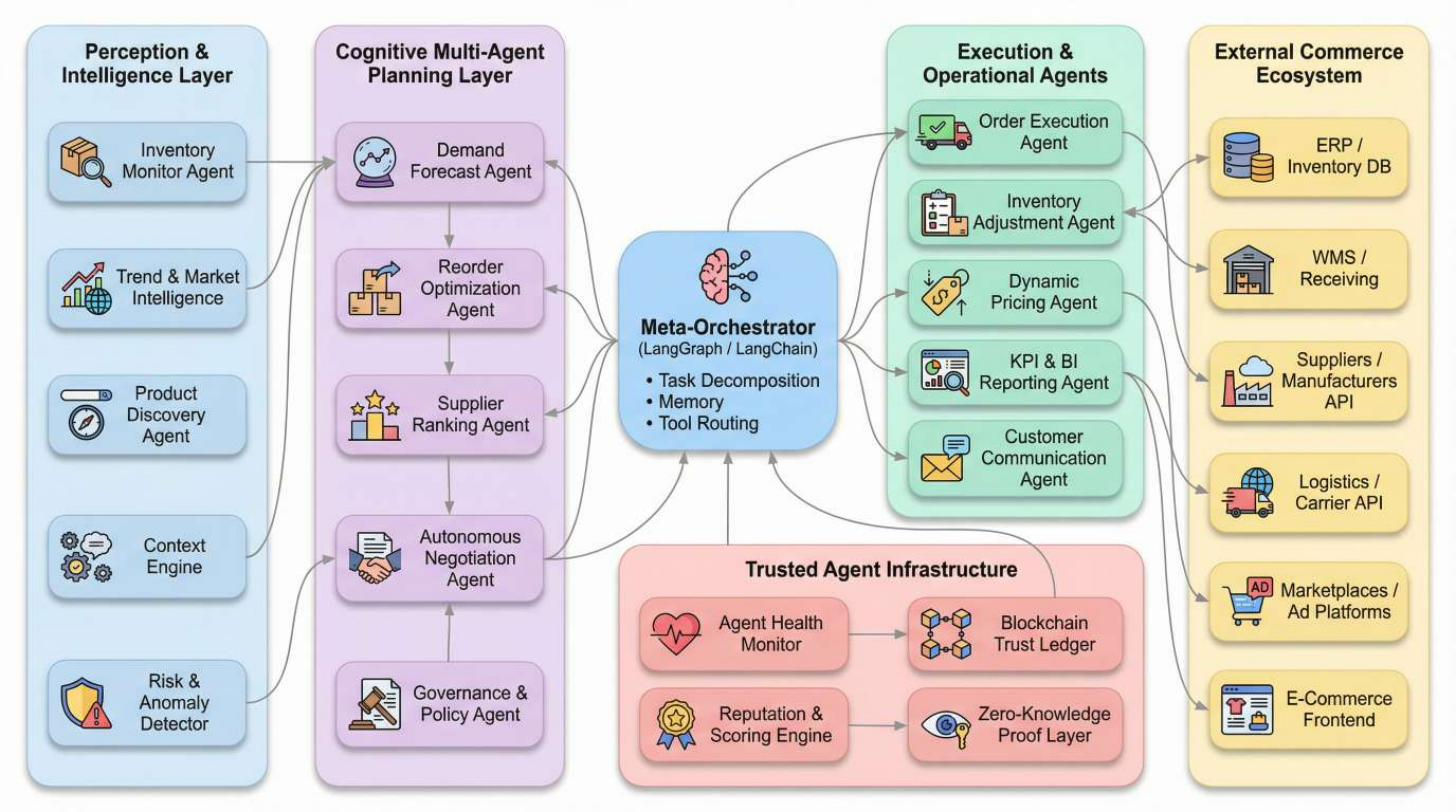
\includegraphics[width=\linewidth]{images/arch-new-V1}
		\caption{Complete architecture of the AAIRM agentic inventory framework.
			The Perception and Intelligence Layer supplies structured context to
			the Cognitive Multi-Agent Planning Layer, which generates replenishment
			and procurement decisions.  A central Meta-Orchestrator
			(LangGraph/LangChain) handles task decomposition, agent memory, and
			tool routing.  Execution and Operational Agents implement approved
			decisions via standardised tool interfaces to the External Commerce
			Ecosystem, while the Trusted Agent Infrastructure provides health
			monitoring, reputation scoring, and cryptographic accountability.}
		\label{fig:pca-arch}
	\end{figure*}

	\subsection{Perception Layer}
	\label{sec:perception}

	The perception layer structures the raw signals required for downstream
	reasoning.  It consists of five specialised agents.

	The \textbf{Inventory Monitor Agent (P1)} periodically queries the
	inventory database, ERP system, and WMS to retrieve on-hand quantities,
	reserved and in-transit stock, inbound purchase orders, and recent receipts
	or shrinkage events.  It applies configurable threshold rules to identify
	SKUs at risk of falling below safety levels or of becoming overstocked,
	and forwards a focused SKU set---with attributes including current location,
	lead-time estimate, and remaining shelf life---to the conceptualization
	layer.

	The \textbf{Trend and Market Intelligence Agent (P2)} monitors external
	signals including search trends, social media activity, and third-party
	marketplace data to identify products or attributes exhibiting strong
	positive momentum or emerging consumer attention.  It produces a ranked
	list of candidate products accompanied by trend-strength scores and
	descriptive features, enabling the framework to anticipate future demand
	rather than solely respond to observed depletion.

	The \textbf{Product Discovery Agent (P3)} cross-references external trend
	signals with the mart's existing assortment to surface new or
	underrepresented SKUs that merit stocking evaluation.  It operates jointly
	with P2 to ensure that the framework's replenishment and procurement scope
	extends beyond the current catalogue.

	The \textbf{Context Engine (P4)} assembles feature-rich contextual
	representations for forecasting and optimisation by combining historical
	sales trajectories with calendar and seasonal effects (holidays,
	promotional windows, weekend patterns), price history, and category-level
	metadata.  This structured perceptual state forms the primary input to the
	conceptualization layer.

	The \textbf{Risk and Anomaly Detector (P5)} identifies irregular
	signals---demand spikes, supplier anomalies, sudden inventory discrepancies,
	or data quality issues---and routes alerts to the Governance Agent (C5) for
	review before any procurement decision is finalised.

	\subsection{Conceptualization Layer}
	\label{sec:conceptualization}

	The conceptualization layer transforms perceived information into
	replenishment and procurement decisions through a combination of predictive
	modelling, multi-objective optimisation, and policy enforcement.  It
	comprises five agents.

	\subsubsection{Demand Forecasting Agent (C1)}

	The Demand Forecasting Agent receives the focused SKU set from P1, trend
	priors from P2--P3, and contextual features from P4.  For each SKU $i$,
	it constructs a feature vector $\mathbf{x}_{i,t}$ at time $t$ and
	estimates future demand over a planning horizon $H$.  Let
	$y_{i,t+h}$ denote demand in period $t+h$.  The forecasting model is
	\begin{equation}
		\label{eq:forecast}
		\hat{y}_{i,t+h} = f_\theta(\mathbf{x}_{i,t},\, h),
	\end{equation}
	where $f_\theta$ is a learned function---specifically, a deep time-series
	architecture with exogenous feature attention (e.g., a Temporal Fusion
	Transformer or LSTM encoder-decoder)---parameterised by $\theta$.
	Training minimises
	\begin{equation}
		\label{eq:loss}
		\mathcal{L}(\theta) =
		\sum_{i,t,h} \ell\!\left(y_{i,t+h},\, f_\theta(\mathbf{x}_{i,t},h)\right),
	\end{equation}
	where $\ell(\cdot)$ is mean squared error for point forecasts or a
	pinball loss for quantile forecasts.  The agent outputs per-SKU point
	forecasts and uncertainty summaries (mean, variance, prediction intervals)
	for use by C2.

	\subsubsection{Reorder Optimisation Agent (C2)}

	The Reorder Optimisation Agent translates forecasts and current inventory
	state into order proposals.  For SKU $i$, let $Q_i$ denote the planned
	order quantity, $\tilde{D}_i$ the random demand during the replenishment
	cycle (derived from the forecast distribution), $c_i$ the unit procurement
	cost, $h_i$ the per-unit holding cost rate, $p_i$ the penalty cost for
	unmet demand, and $\delta_i$ the spoilage cost rate for perishables.  The
	single-period expected cost is
	\begin{equation}
		\label{eq:cost}
		\begin{aligned}
			C_i(Q_i) \;=\;&
			c_i Q_i
			+ h_i\,\mathbb{E}\!\left[(Q_i - \tilde{D}_i)_+\right]\\
			&+\; p_i\,\mathbb{E}\!\left[(\tilde{D}_i - Q_i)_+\right]
			+ \delta_i\,\mathbb{E}\!\left[\max\!\left\{0,\,Q_i - \tilde{D}_i^{\text{life}}\right\}\right],
		\end{aligned}
	\end{equation}
	where $(x)_+ = \max(0,x)$ and $\tilde{D}_i^{\text{life}}$ is the demand
	realisable within the effective shelf-life window.  The agent solves the
	constrained cost-minimisation problem
	\begin{equation}
		\label{eq:optim}
		\min_{Q_i \ge 0}\; \sum_{i} C_i(Q_i)
		\quad\text{subject to}\quad
		\sum_i c_i Q_i \le B,\quad
		\sum_i v_i Q_i \le V,
	\end{equation}
	where $B$ is the purchasing budget and $v_i$ is the volumetric footprint
	per unit of SKU $i$, bounded by warehouse capacity $V$.

	In multi-period settings the agent learns a policy
	$\pi_\phi : \mathcal{S} \to \mathcal{A}$ that maps the system state $s_t$
	(current inventory, forecasts, trend signals) to order actions $a_t$ by
	maximising the expected discounted return:
	\begin{equation}
		\label{eq:rl}
		\max_{\pi_\phi}\;\mathbb{E}\!\left[\sum_{t=0}^{\infty}\gamma^{t}\,r(s_t,a_t)\right],
	\end{equation}
	where $\gamma \in (0,1)$ is a discount factor and the reward
	$r(\cdot,\cdot)$ equals the negative expected cost in
	Eq.~(\ref{eq:cost}).  Policy optimisation is implemented via Proximal
	Policy Optimisation (PPO), which provides stable gradient updates and
	handles the continuous action space of order quantities without requiring
	explicit model-based planning.  This RL formulation enables the agent to
	adapt to non-stationary demand and evolving lead-time distributions without
	re-specification of fixed thresholds.

	\subsubsection{Supplier Ranking Agent (C3)}

	For each $(i, Q_i)$ pair approved by C2, the Supplier Ranking Agent
	queries supplier catalogues to collect feasible offers.  Let
	$\mathcal{S}_i$ be the set of qualified suppliers for SKU $i$, and let
	supplier $j \in \mathcal{S}_i$ be characterised by unit cost $c_{ij}$,
	promised lead time $L_{ij}$, historical reliability $r_{ij}$, and minimum
	order quantity $m_{ij}$.  A composite score is computed as
	\begin{equation}
		\label{eq:supplier}
		\text{Score}_{ij} =
		\alpha_1 c_{ij}
		+ \alpha_2 \hat{L}_{ij}
		- \alpha_3 r_{ij}
		+ \alpha_4\,\mathbb{I}\{Q_i < m_{ij}\},
	\end{equation}
	where $\hat{L}_{ij}$ incorporates historical lead-time deviations and
	$\alpha_1,\dots,\alpha_4$ are tunable weights.  Suppliers are ranked in
	ascending order of $\text{Score}_{ij}$, and a shortlist of top candidates
	is forwarded to the Autonomous Negotiation Agent (C4) and the Governance
	Agent (C5).

	\subsubsection{Autonomous Negotiation Agent (C4)}

	The Autonomous Negotiation Agent receives supplier shortlists from C3
	and engages in structured dialogue with supplier systems to elicit revised
	quotations, request volume discounts, or propose alternative delivery
	schedules.  Following negotiation, the agent finalises commercial
	terms---quantity, unit price, delivery window, and payment conditions---and
	routes confirmed proposals to C5 and, upon governance approval, to the
	Order Execution Agent (A1) for execution.

	\subsubsection{Governance and Policy Agent (C5)}

	The Governance Agent acts as policy enforcer and cross-category coordinator.
	It validates proposed orders from C2, supplier rankings from C3, and
	negotiated terms from C4 against global constraints including category-level
	budget caps, risk-diversification guidelines, and temperature-zone storage
	capacities (e.g., frozen versus ambient goods).  Conflict resolution may
	involve quantity adjustments, supplier substitutions, or order deferrals.
	The output of this agent is an approved set of purchase decisions, annotated
	with binding constraints and priority flags, which is passed to the action
	layer.

	\subsection{Action Layer and Learning Loop}
	\label{sec:action}

	The action layer implements approved plans and closes the learning loop by
	feeding operational outcomes back to the perception and conceptualization
	layers.

	The \textbf{Order Execution Agent (A1)} translates approved purchase
	decisions into purchase orders transmitted to supplier platforms, arranges
	shipments with logistics carriers, and generates receiving operations in the
	WMS.  It processes advanced shipping notices and goods-receipt confirmations,
	updating ERP and inventory databases in real time and propagating key
	performance indicators to the BI reporting layer.

	The \textbf{Inventory Adjustment Agent (A2)} reconciles physical receiving
	events with system records, posting receipt quantities and adjusting
	on-hand balances to reflect actual deliveries.  It also handles short
	shipments, quality rejections, and substitution events, ensuring that the
	perceptual state available to P1 and P4 remains accurate.

	The \textbf{Learning Agent (A3)} sustains continuous improvement of the
	framework by collecting event streams including realised lead times,
	delivery deviations, stockout events, wastage, and demand surprises.  This
	data is used to retrain demand forecasting models
	(Eq.~\ref{eq:forecast}), recalibrate cost and spoilage parameters
	(Eq.~\ref{eq:cost}), and refine supplier reliability estimates
	(Eq.~\ref{eq:supplier}).  In RL variants, the learning agent updates the
	policy parameters $\phi$ of C2 by minimising a temporal-difference loss:
	\begin{equation}
		\label{eq:td}
		\mathcal{L}_{\text{TD}}(\phi) =
		\left(r_t + \gamma\,V_\phi(s_{t+1}) - V_\phi(s_t)\right)^2,
	\end{equation}
	where $V_\phi(s)$ is an approximate value function.  Through this feedback
	loop the framework progressively adapts to shifts in consumer behaviour,
	supplier performance, and operational constraints.

	Beyond the core PCA agents, the architecture includes complementary
	operational agents visible in Figure~\ref{fig:pca-arch}: a \textbf{Dynamic
	Pricing Agent} that adjusts shelf prices in response to inventory levels and
	competitor signals, a \textbf{KPI and BI Reporting Agent} that aggregates
	performance metrics for managerial dashboards, and a \textbf{Customer
	Communication Agent} that generates fulfilment and availability
	notifications.  While these agents are integral to the full production
	deployment, the empirical evaluation in Section~\ref{sec:impl} focuses on
	the core replenishment and procurement pipeline (P1--P5, C1--C5, A1--A3).

	The \textbf{Trusted Agent Infrastructure} underpins the entire system with
	an Agent Health Monitor that detects and isolates failing or anomalous
	agents, a Reputation and Scoring Engine that maintains longitudinal
	performance records for each agent and supplier, a Blockchain Trust Ledger
	that provides an immutable audit trail of all procurement events, and a
	Zero-Knowledge Proof Layer that enables privacy-preserving verification of
	commercial terms.  These components collectively ensure accountability,
	auditability, and resilience in a fully autonomous procurement environment.

	\subsection{Use-Case: Execution Flow}
	\label{sec:sequence}

	Figure~\ref{fig:sequence-diagram} illustrates the end-to-end execution
	flow for a low-stock replenishment event in the proposed AAIRM system,
	tracing how an unstructured user request is transformed into a confirmed
	purchase order through the integrated PCA pipeline.

	\begin{figure*}[htbp]
		\centering
		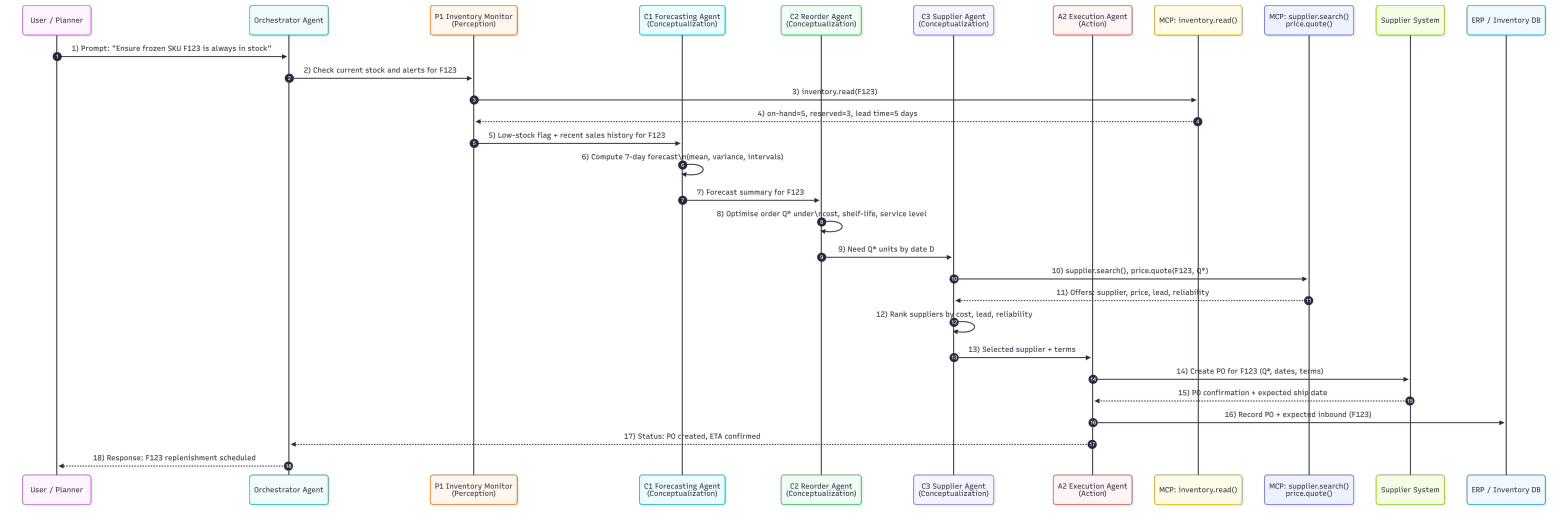
\includegraphics[width=\linewidth]{images/sequence-use-case}
		\caption{Sequence and use-case execution flow of the AAIRM framework
			for a low-stock replenishment event (SKU F123, frozen category).
			The diagram traces all 18 interaction steps from the user prompt
			through perception, conceptualization, and action
			layers---including MCP tool calls to the inventory database and
			supplier systems---to final ERP synchronisation and user
			confirmation.}
		\label{fig:sequence-diagram}
	\end{figure*}

	The process is initiated when the user issues a natural-language instruction
	to ensure the availability of a specific SKU (frozen product F123).  The
	Meta-Orchestrator interprets the request and dispatches it to the Inventory
	Monitor (P1), which queries the inventory management system via an MCP call
	and retrieves the on-hand quantity (five units), reserved stock (three
	units), and estimated lead time (five days), confirming a low-stock
	condition.

	Upon low-stock detection, P1 forwards the SKU identifier and recent sales
	history to the Demand Forecasting Agent (C1), which computes a 7-day demand
	forecast including mean, variance, and confidence intervals.  The forecast
	is relayed to the Reorder Optimisation Agent (C2), which calculates the
	optimal replenishment quantity $Q^*$ subject to cost parameters, lead-time
	uncertainty, shelf-life constraints, and service-level targets
	(Eq.~\ref{eq:optim}).

	C2 issues a procurement request to the Supplier Ranking Agent (C3),
	specifying $Q^*$ and the required delivery window.  C3 queries external
	supplier catalogues via MCP tools, collects quotations on price,
	availability, lead time, and reliability, and ranks candidates using
	Eq.~(\ref{eq:supplier}).  The top-ranked supplier and associated commercial
	terms are forwarded to the Order Execution Agent (A1).

	A1 transmits the purchase order to the selected supplier, receives a
	purchase order confirmation along with the expected ship date, and posts
	the inbound order and anticipated receiving schedule to the ERP and
	inventory database.  Finally, the Meta-Orchestrator returns a summary of
	the approved purchase order and replenishment schedule to the user,
	completing the Perception--Conceptualization--Action cycle.

	% -------------------------------------------------------
	\section{Experimental Setup and Results}
	\label{sec:impl}

	\subsection{Experimental Environment}

	The AAIRM framework was deployed as an agentic application in which each
	logical agent---Inventory Monitor, Demand Forecasting, Reorder Optimisation,
	Supplier Ranking, Governance, Negotiation, Execution, and Learning---was
	instantiated as a discrete LangChain agent with a defined tool set.  Tools
	expose enterprise systems and external platforms through a common interface
	layer comprising an inventory and sales database connector, a supplier
	catalogue query service, a logistics API stub, and a warehouse management
	system adapter.  Each agent's reasoning and planning logic is supported by
	a commercial instruction-tuned LLM; numerical forecasting models and
	optimisation routines are implemented in Python and invoked as tools.

	To evaluate the framework under realistic but controlled conditions, we
	constructed a synthetic retail environment comprising 1\,200 SKUs
	distributed across five product categories: grocery, frozen food, apparel,
	cosmetics, and dry fruits (240 SKUs per category).  Demand was simulated
	over a two-year horizon for each SKU using a process incorporating
	category-specific base demand profiles, weekly seasonality, promotional
	uplifts, and independent random shocks.  Perishable SKUs (frozen goods and
	selected cosmetics) were assigned category-specific shelf lives and
	temperature-zone capacity constraints.  Lead times and supplier reliability
	scores were sampled from empirically calibrated distributions, and three to
	five suppliers were generated per SKU with heterogeneous pricing and minimum
	order quantities.

	All experiments were conducted in an offline controlled setting.  LangChain
	agents communicated with a simulated backend that reproduced the behaviour
	of ERP, WMS, and supplier systems---including delayed shipments, sporadic
	supplier-side stockouts, and noisy acknowledgements.  This configuration
	enabled the evaluation of complex operational scenarios with full
	ground-truth control over demand and cost structures, without requiring
	access to proprietary production data.

	\subsection{Baselines and Evaluation Metrics}

	The AAIRM system was compared against two baselines representative of
	common industry practices.  \textbf{Baseline~1 (ROP--EOQ)} is a traditional
	reorder-point and economic-order-quantity policy in which demand means and
	variances were estimated from historical sales and a fixed safety factor
	was applied to achieve a nominal service level; orders were triggered
	whenever available stock fell below the computed reorder point.
	\textbf{Baseline~2 (ML + Static Policy)} is a non-agentic system in which
	a global gradient-boosted tree model provided daily demand forecasts, but
	order logic remained rule-based; forecasts were recomputed daily, but there
	was no supplier negotiation and no cross-category coordination.

	Performance was evaluated over a one-year test horizon on five metrics:
	(i)~\emph{stockout rate} (percentage of demand not satisfied from on-hand
	inventory); (ii)~\emph{fill rate} (fraction of line items fully satisfied
	on time); (iii)~\emph{average inventory} (mean on-hand units normalised by
	demand); (iv)~\emph{total cost} (sum of procurement, holding, penalty, and
	spoilage costs, normalised to Baseline~1); and (v)~\emph{supplier
	diversification index} (a concentration measure penalising over-reliance
	on a single supplier per category, scaled to $[0,1]$ with higher values
	indicating greater diversification).

	\subsection{Quantitative Results}

	Table~\ref{tab:results-overview} summarises overall performance across all
	categories.  AAIRM achieves the lowest stockout rate (3.9\%), the highest
	fill rate (97.8\%), and the lowest total cost (0.84, normalised) of all
	three policies, while also maintaining the leanest average inventory (1.19
	units per unit of demand) and the highest supplier diversification index
	(0.61).

	\begin{table*}[htbp]
		\centering
		\caption{Performance comparison across the three inventory policies
			over the one-year test horizon.  Total cost and average inventory
			are normalised to Baseline~1.  Supplier diversification index is
			scaled to $[0,1]$; higher values indicate lower single-source
			concentration.}
		\label{tab:results-overview}
		\begin{tabular}{lccccc}
			\toprule
			\textbf{Policy}
			& \textbf{Stockout (\%)}
			& \textbf{Fill Rate (\%)}
			& \textbf{Avg.\ Inv.}
			& \textbf{Total Cost}
			& \textbf{Div.\ Index} \\
			\midrule
			Baseline~1 (ROP--EOQ)          & 8.7 & 93.1 & 1.45 & 1.00 & 0.42 \\
			Baseline~2 (ML + Static)       & 6.2 & 95.4 & 1.32 & 0.93 & 0.47 \\
			AAIRM (proposed)               & \textbf{3.9} & \textbf{97.8}
			                               & \textbf{1.19} & \textbf{0.84}
			                               & \textbf{0.61} \\
			\bottomrule
		\end{tabular}
	\end{table*}

	Table~\ref{tab:results-category} presents the per-category breakdown of
	AAIRM performance and the corresponding Baseline~1 figures.  Frozen food
	and dry fruits exhibit the highest stockout rates across all conditions,
	reflecting the compounded difficulty of perishability constraints and
	less predictable consumption patterns.  Apparel benefits from the most
	stable demand seasonality and accordingly shows the strongest stockout
	reduction (from 6.5\% to 2.8\%).  The spoilage column---applicable only
	to perishable categories---shows that AAIRM substantially reduces wastage
	relative to the static baseline by tightening order quantities to align
	with shelf-life windows, consistent with the optimisation formulation in
	Eq.~(\ref{eq:cost}).

	\begin{table*}[htbp]
		\centering
		\caption{Per-category performance comparison between AAIRM and
			Baseline~1 (ROP--EOQ) over the one-year test horizon.
			Spoilage rate is reported only for perishable categories (frozen
			food, cosmetics, and dry fruits); \textemdash~indicates not
			applicable.}
		\label{tab:results-category}
		\begin{tabular}{lcccccc}
			\toprule
			\multirow{2}{*}{\textbf{Category}}
			& \multicolumn{2}{c}{\textbf{Stockout (\%)}}
			& \multicolumn{2}{c}{\textbf{Fill Rate (\%)}}
			& \multicolumn{2}{c}{\textbf{Spoilage (\%)}} \\
			\cmidrule(lr){2-3}\cmidrule(lr){4-5}\cmidrule(lr){6-7}
			& BL-1 & AAIRM & BL-1 & AAIRM & BL-1 & AAIRM \\
			\midrule
			Grocery      & 7.4  & 3.2  & 93.8 & 98.1 & \textemdash & \textemdash \\
			Frozen food  & 11.8 & 4.9  & 90.2 & 96.9 & 6.3         & 2.8 \\
			Apparel      & 6.5  & 2.8  & 94.4 & 98.7 & \textemdash & \textemdash \\
			Cosmetics    & 9.1  & 4.3  & 92.1 & 97.4 & 3.7         & 1.6 \\
			Dry fruits   & 8.7  & 4.3  & 93.1 & 97.9 & 4.1         & 2.0 \\
			\midrule
			\textbf{Overall} & \textbf{8.7} & \textbf{3.9} &
			                   \textbf{93.1} & \textbf{97.8} & \textemdash & \textemdash \\
			\bottomrule
		\end{tabular}
	\end{table*}

	Figure~\ref{fig:results-bar} presents a normalised visual comparison of
	stockout rate, total cost, and average inventory across the three policies.
	Each metric is expressed relative to Baseline~1.  AAIRM reduces the
	stockout rate by 55.2\% relative to the ROP--EOQ baseline and by 37.1\%
	relative to the ML + Static policy, and achieves a 16\% reduction in total
	cost over Baseline~1.  The improvement in supplier diversification (from
	0.42 to 0.61) reflects the Supplier Ranking and Negotiation Agents'
	tendency to distribute procurement volume across multiple suppliers,
	mitigating single-source concentration risk.

	\begin{figure}[htbp]
		\centering
		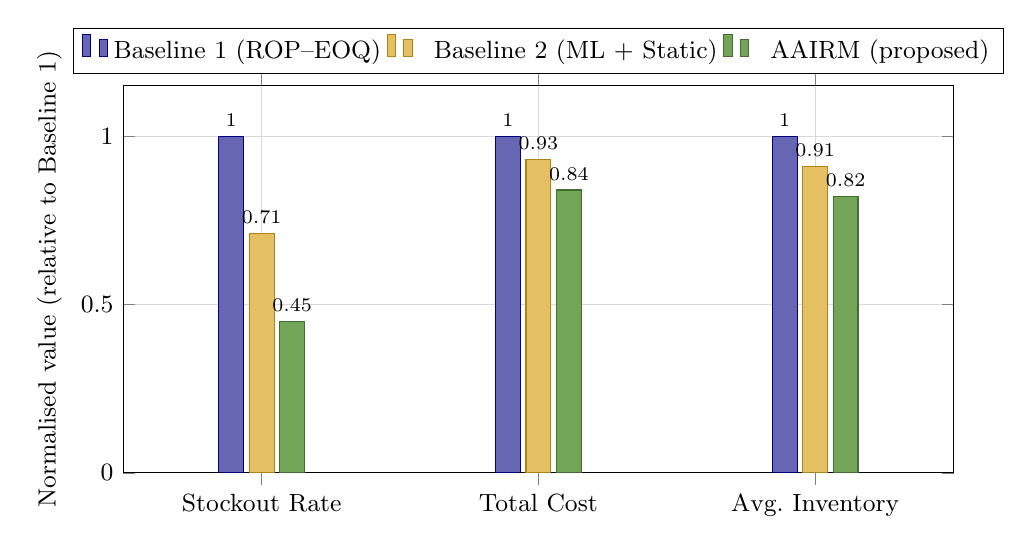
\begin{tikzpicture}
			\begin{axis}[
				ybar,
				bar width=9pt,
				width=\linewidth,
				height=6.5cm,
				enlarge x limits=0.25,
				ymin=0, ymax=1.15,
				ylabel={Normalised value (relative to Baseline~1)},
				symbolic x coords={Stockout Rate, Total Cost, Avg.\ Inventory},
				xtick=data,
				legend style={at={(0.5,1.03)}, anchor=south, legend columns=-1,
					font=\small},
				nodes near coords,
				nodes near coords style={font=\scriptsize,
					/pgf/number format/fixed,
					/pgf/number format/precision=2},
				tick label style={font=\small},
				label style={font=\small},
				grid=both,
				grid style={line width=0.3pt, draw=gray!30},
				]
				\addplot[fill=NavyBlue!60, draw=NavyBlue]
				coordinates {(Stockout Rate,1.00)(Total Cost,1.00)(Avg.\ Inventory,1.00)};
				\addplot[fill=Goldenrod!70, draw=Goldenrod!80!black]
				coordinates {(Stockout Rate,0.71)(Total Cost,0.93)(Avg.\ Inventory,0.91)};
				\addplot[fill=OliveGreen!65, draw=OliveGreen!80!black]
				coordinates {(Stockout Rate,0.45)(Total Cost,0.84)(Avg.\ Inventory,0.82)};
				\legend{Baseline~1 (ROP--EOQ),\; Baseline~2 (ML + Static),\; AAIRM (proposed)}
			\end{axis}
		\end{tikzpicture}
		\caption{Normalised comparison of stockout rate, total cost, and
			average inventory across the three policies.  All values are
			divided by the corresponding Baseline~1 value.  AAIRM achieves
			the lowest normalised value on all three metrics.}
		\label{fig:results-bar}
	\end{figure}

	Figure~\ref{fig:rl-training} shows the learning curve of the Reorder
	Optimisation Agent (C2) during simulated RL training.  The average episode
	cost decreases steadily from 1.00 (initial random policy) and stabilises
	at approximately 0.82 after 250 episodes, demonstrating policy convergence.
	The convergence profile confirms that the agent learns to balance ordering
	frequency and quantity against holding costs and stockout penalties within
	the simulated environment.

	\begin{figure}[htbp]
		\centering
		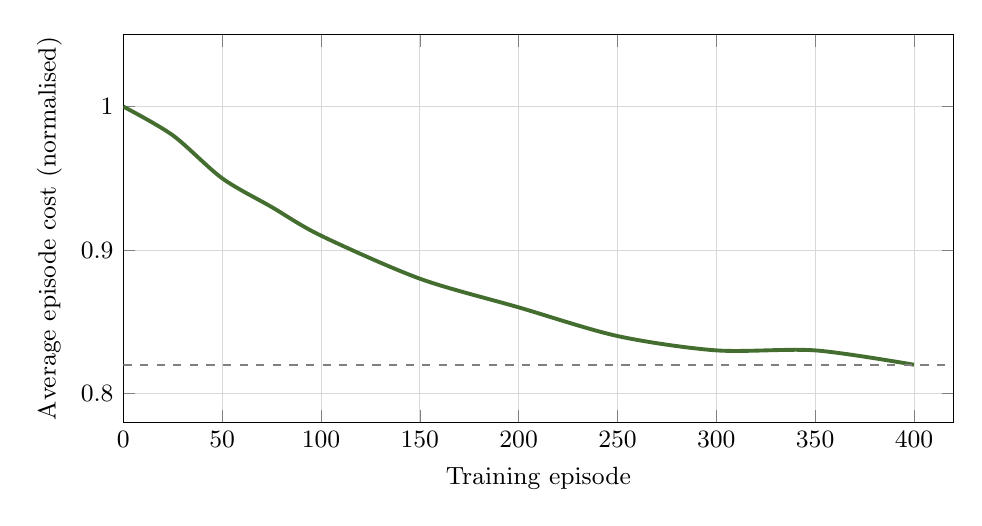
\begin{tikzpicture}
			\begin{axis}[
				width=\linewidth,
				height=6.5cm,
				xlabel={Training episode},
				ylabel={Average episode cost (normalised)},
				xmin=0, xmax=420,
				ymin=0.78, ymax=1.05,
				grid=both,
				grid style={line width=0.3pt, draw=gray!30},
				tick label style={font=\small},
				label style={font=\small},
				]
				\addplot[smooth, thick, color=OliveGreen!80!black, line width=1.4pt]
				coordinates {
					(0,1.00) (25,0.98) (50,0.95) (75,0.93)
					(100,0.91) (150,0.88) (200,0.86) (250,0.84)
					(300,0.83) (350,0.83) (400,0.82)
				};
				\draw[dashed, gray, line width=0.8pt]
				(axis cs:0,0.82) -- (axis cs:420,0.82)
				node[right, font=\scriptsize] {$\approx 0.82$};
			\end{axis}
		\end{tikzpicture}
		\caption{Training curve for the Reorder Optimisation Agent (C2)
			in the simulated environment.  The average normalised cost per
			episode decreases monotonically and converges to approximately
			0.82 by episode~250, indicating stable policy learning.}
		\label{fig:rl-training}
	\end{figure}

	\subsection{Qualitative Observations}

	Inspection of individual replenishment curves reveals category-level
	behavioural differences that illustrate the value of the integrated PCA
	architecture.  For fast-moving grocery SKUs with short, reliable lead
	times, AAIRM adopts a high-frequency, small-batch ordering strategy that
	keeps average inventory lean without incurring stockout penalties.  For
	frozen and other perishable SKUs, the policy shifts toward higher safety
	stock but tighter shelf-life alignment, reducing wastage relative to the
	overstocking tendency observed in both baselines (Table~\ref{tab:results-category}).
	Notably, the Supplier Ranking and Negotiation Agents dynamically redirect
	procurement volume away from suppliers whose recent lead-time performance
	has deteriorated---even when the nominal quoted price remains
	attractive---a behaviour that is structurally impossible to encode in static
	threshold-based policies.  These emergent behaviours demonstrate that the
	benefits of AAIRM derive from the coordinated integration of perception,
	conceptualization, and action, and cannot be replicated by any
	single-component improvement in isolation.

	% -------------------------------------------------------
	\section{Discussion}
	\label{sec:discussion}

	\subsection{Economic Implications of Agentic Procurement Automation}

	The quantitative results underscore the economic case for agentic AI in
	retail inventory management.  A 16\% reduction in total operational cost
	and a 55.2\% reduction in the stockout rate, relative to the
	industry-standard ROP--EOQ baseline, translate directly into lower
	lost-sales revenue and reduced capital tied up in excess stock.  The
	improvement in supplier diversification from 0.42 to 0.61 represents a
	structural risk reduction: by distributing procurement volume across
	multiple suppliers, AAIRM limits exposure to single-source disruptions of
	the kind that created severe supply-chain vulnerabilities in global retail
	during 2020--2022.  For large multi-category marts handling thousands of
	SKUs, even marginal per-unit cost improvements aggregate into substantial
	annual savings.  The per-category breakdown (Table~\ref{tab:results-category})
	further reveals that the gains are not uniform: the largest absolute
	improvements occur in frozen food, the most operationally constrained
	category, where shelf-life alignment and responsive supplier switching
	deliver disproportionate waste and stockout reductions.  The proposed
	framework positions agentic AI not merely as an operational efficiency
	tool but as a source of strategic economic value through adaptive risk
	management and responsive procurement.

	\subsection{Deployment Considerations}

	Several practical factors condition the successful deployment of AAIRM
	in live retail environments.

	\textbf{LLM inference latency.}  Each agent in the AAIRM stack invokes an
	LLM for reasoning and planning.  In time-sensitive replenishment
	scenarios---particularly for fast-moving perishables---inference latency
	must be managed carefully.  Asynchronous agent execution, caching of
	repeated tool calls, and the use of smaller distilled models for routine
	sub-tasks are practical mitigation strategies; however, their interaction
	with decision quality has not been evaluated in the present study.

	\textbf{Supplier API standardisation.}  The framework assumes programmatic
	access to supplier catalogues for price queries and order placement.  In
	practice, supplier systems vary widely in API maturity: some expose
	structured REST interfaces, while others rely on EDI formats or
	email-based workflows.  An MCP translation layer or a supervised supplier
	onboarding process is required to bridge this heterogeneity.

	\textbf{ERP and WMS integration.}  Tight integration with ERP and WMS
	systems is necessary for the perception agents to maintain accurate,
	real-time inventory state.  Latency or inconsistency in these data feeds
	can propagate errors through the entire PCA pipeline.  Robust data quality
	monitoring---partially addressed by the Risk and Anomaly Detector
	(P5)---is therefore a prerequisite for deployment.

	\textbf{Cold-start and sparse-data SKUs.}  Demand forecasting for new or
	infrequently ordered SKUs suffers from sparse historical data, a challenge
	not fully addressed in the present evaluation.  Transfer learning across
	category hierarchies or Bayesian prior elicitation from similar SKUs are
	candidate solutions that warrant further study.

	\subsection{Limitations}

	The present work has several limitations that bound the scope of its
	conclusions.

	\textbf{Simulation-based evaluation.}  The experimental results were
	obtained entirely in a synthetic simulation.  While the simulation was
	calibrated to realistic demand and supply parameters, it does not capture
	the full complexity of live retail operations, including real-time data
	quality issues, adversarial supplier behaviour, and emergent interactions
	between categories.  Field deployment on a real mart---even in a shadow
	mode that logs agentic decisions without acting on them---would provide
	substantially stronger evidence of practical utility.

	\textbf{Synthetic data generation.}  Because the framework was evaluated on
	data generated under a known stochastic model, the forecasting agents have
	an inherent structural advantage over the baselines.  An evaluation on
	genuinely observed retail scanner data would provide a more demanding and
	externally valid test.

	\textbf{LLM reasoning under adversarial inputs.}  The robustness of
	LLM-based agents to anomalous or adversarial inputs from supplier
	systems---such as inflated quotations, fabricated shipping confirmations,
	or prompt-injection-style attacks on natural-language interfaces---has not
	been assessed.  The Trusted Agent Infrastructure
	(Section~\ref{sec:action}) provides partial mitigation through the Agent
	Health Monitor and the Zero-Knowledge Proof Layer; however, formal security
	analysis of the agentic pipeline remains an open problem.

	\textbf{Computational costs.}  The per-decision cost of running multiple
	LLM-backed agents in a production environment has not been quantified.  For
	marts with very large SKU counts, the inference budget may be a binding
	operational constraint.

	\subsection{Governance and Human-AI Trust}

	Autonomous procurement decisions carry financial and legal consequences that
	necessitate clearly defined human oversight mechanisms.  The Governance and
	Policy Agent (C5) and the Blockchain Trust Ledger provide auditability and
	constraint enforcement within the agentic pipeline, but they do not
	substitute for human governance structures at the organisational level.
	Retailers deploying AAIRM should establish explicit escalation
	thresholds---for example, requiring human approval for orders exceeding a
	specified monetary value or sourced from a new, unverified supplier---and
	should audit the system's procurement decisions periodically to detect
	systematic biases or policy drift.  Transparency mechanisms such as decision
	summaries generated by the Meta-Orchestrator (as illustrated in the sequence
	diagram, Figure~\ref{fig:sequence-diagram}) are a prerequisite for building
	practitioner trust in agentic procurement automation.

	% -------------------------------------------------------
	\section{Conclusion}
	\label{sec:conclusion}

	This paper presented AAIRM, an agentic AI framework for autonomous inventory
	replenishment and product discovery in multi-category retail environments.
	By organising specialised agents across a structured
	Perception--Conceptualization--Action pipeline---coordinated by a central
	Meta-Orchestrator and supported by a Trusted Agent Infrastructure---the
	framework integrates real-time inventory monitoring, multi-horizon demand
	forecasting, constrained reorder optimisation, multi-criteria supplier
	ranking, autonomous negotiation, and learning from operational feedback into
	a cohesive decision loop.

	Simulation experiments over 1\,200 SKUs and five product categories
	demonstrate that AAIRM reduces the stockout rate from 8.7\% to 3.9\%
	(a 55.2\% relative improvement), lowers total operational cost by 16\%,
	raises the fill rate to 97.8\%, and substantially improves supplier
	diversification relative to both a classical ROP--EOQ policy and a
	non-agentic ML baseline.  Per-category analysis further reveals that the
	gains are largest in operationally constrained categories such as frozen
	food, where combined shelf-life management and dynamic supplier switching
	deliver disproportionate reductions in both stockouts and wastage.  These
	gains are attributable to the framework's ability to combine heterogeneous
	data sources, reason under operational constraints, and adapt dynamically
	to changing demand and supplier behaviour---capabilities that static
	policies cannot replicate.

	Future work should prioritise three directions.  First, field deployment on
	live retail data is necessary to validate the simulation findings and to
	characterise real-world failure modes.  Second, security and robustness
	analysis of the agentic pipeline---including adversarial resilience and
	formal verification of governance constraints---requires dedicated
	investigation.  Third, the framework should be extended to incorporate
	dynamic pricing agents and customer demand shaping, enabling end-to-end
	margin optimisation that integrates replenishment and revenue management
	within a single agentic system.

	% -------------------------------------------------------
	\medskip
	\begin{thebibliography}{99}

		\bibitem{mckinsey2024retailai}
		McKinsey \& Company, ``The 2024 Global Retail AI Index: Capturing the
		\$1.8 Trillion Efficiency Gap,'' \emph{McKinsey Insights}, 2024.
		Available: \url{https://www.mckinsey.com/industries/retail/our-insights}
		(accessed 15 November 2025).

		\bibitem{capgemini2023autonomous}
		Capgemini Research Institute, ``Autonomous Supply Chains: The Next
		Frontier in Retail,'' Capgemini White Paper, 2023.
		Available: \url{https://www.capgemini.com/research/autonomous-supply-chains/}
		(accessed 15 November 2025).

		\bibitem{bullwhip2007effect}
		H.~L.\ Lee, V.~Padmanabhan, and S.~Whang,
		\emph{The Bullwhip Effect in Supply Chains}.
		Cambridge, MA: MIT Press, 2007.

		\bibitem{jannelli2024agentic}
		M.~Jannelli, R.~Schaefer, and L.~Zhang,
		``Agentic LLMs in the Supply Chain: Consensus-Seeking Agents for
		Procurement and Planning,''
		\emph{arXiv preprint arXiv:2411.10184}, 2024.

		\bibitem{culot2024ai}
		G.~Culot, G.~Orzes, and M.~Sartor,
		``Artificial Intelligence Applications in Supply Chain and Inventory
		Management: A Systematic Review,''
		\emph{Journal of Purchasing and Supply Management}, Elsevier, 2024.

		\bibitem{yilmaz2024aiinventory}
		E.~Y{\i}lmaz, M.~Karakaya, and U.~Kose,
		``AI-Driven Optimization of Order Procurement and Inventory Management
		in Supply Chains,''
		\emph{ResearchGate Preprint}, 2024.

		\bibitem{nahmias2019production}
		S.~Nahmias and T.~L.\ Olsen,
		\emph{Production and Operations Analysis}, 8th~ed.
		Long Grove, IL: Waveland Press, 2019,
		ISBN: 978-1-4786-3848-6.

		\bibitem{axsater2015inventory}
		S.~Axs\"{a}ter,
		\emph{Inventory Control}, 3rd~ed.
		Cham: Springer, 2015,
		doi: \href{https://doi.org/10.1007/978-3-319-15729-0}{10.1007/978-3-319-15729-0}.

		\bibitem{sari2008collaborative}
		K.~Sari,
		``On the Benefits of CPFR and VMI: A Comparative Simulation Study,''
		\emph{International Journal of Production Economics},
		vol.~113, no.~2, pp.~575--586, 2008,
		doi: \href{https://doi.org/10.1016/j.ijpe.2007.10.021}{10.1016/j.ijpe.2007.10.021}.

		\bibitem{duan2022iot}
		L.~Duan, Y.~Chen, and Q.~Zhang,
		``IoT-Enabled Autonomous Replenishment for Smart Retail Environments,''
		\emph{IEEE Internet of Things Journal},
		vol.~9, no.~15, pp.~13784--13796, 2022.

		\bibitem{siems2023interpretable}
		J.~Siems and J.~Peters,
		``Interpretable Reinforcement Learning via Neural Additive Models for
		Inventory Management,''
		\emph{arXiv preprint arXiv:2303.10382}, 2023.

		\bibitem{chen2020multiproduct}
		H.~Chen and Z.~Zhang,
		``Reinforcement Learning for Multi-Product Multi-Node Inventory
		Management,''
		\emph{arXiv preprint arXiv:2006.04037}, 2020.

		\bibitem{bhavikatta2024survey}
		P.~Bhavikatta and V.~Reddy,
		``A Comprehensive Survey of AI-Based Inventory Optimization Systems,''
		\emph{Journal of Computer Science and Technology Studies},
		vol.~6, no.~2, pp.~1--14, 2024.

		\bibitem{shen1999multiagent}
		W.~Shen and D.~H.\ Norrie,
		``Agent-Based Systems for Intelligent Manufacturing: A State-of-the-Art
		Survey,''
		\emph{Knowledge and Information Systems},
		vol.~1, no.~2, pp.~129--156, 1999,
		doi: \href{https://doi.org/10.1007/BF03325096}{10.1007/BF03325096}.

		\bibitem{davidrajuh2018multiagent}
		R.~Davidrajuh and B.~Lin,
		``A Multi-Agent Simulation Approach for Dynamic Inventory Balancing in
		Supply Chains,''
		\emph{Procedia Computer Science},
		vol.~141, pp.~113--120, 2018,
		doi: \href{https://doi.org/10.1016/j.procs.2018.10.157}{10.1016/j.procs.2018.10.157}.

		\bibitem{nahmias1982perishable}
		S.~Nahmias,
		``Perishable Inventory Theory: A Review,''
		\emph{Operations Research},
		vol.~30, no.~4, pp.~680--708, 1982,
		doi: \href{https://doi.org/10.1287/opre.30.4.680}{10.1287/opre.30.4.680}.

		\bibitem{karaesmen2011perishable}
		I.~Z.\ Karaesmen, A.~Scheller-Wolf, and G.-J.\ Van Houtum,
		``Managing Perishable and Aging Inventories: Review and Future Research
		Directions,''
		in \emph{Planning Production and Inventories in the Extended Enterprise},
		K.~G.\ Kempf, P.~Keskinocak, and R.~Uzsoy, Eds.
		New York: Springer, 2011, pp.~393--436,
		doi: \href{https://doi.org/10.1007/978-1-4419-6485-4_15}{10.1007/978-1-4419-6485-4\_15}.

		\bibitem{shukla2023review}
		P.~Shukla and I.~Bose,
		``A Review of Deep Learning in Supply Chain Management: Trends,
		Opportunities, and Challenges,''
		\emph{International Journal of Production Research},
		vol.~61, no.~7, pp.~2123--2142, 2023,
		doi: \href{https://doi.org/10.1080/00207543.2022.2096882}{10.1080/00207543.2022.2096882}.

	\end{thebibliography}

\end{document}
